\section{Lecture 1: Principal Component Analysis}

Principal Component Analysis (PCA), also known as the Karhunen--Loeve transform, is the first projection method in Machine Intelligence II. The problem starts with observations
\[
  x^{(\alpha)} \in \mathbb{R}^N,
  \qquad \alpha = 1,\dots,p,
\]
and asks which directions in feature space expose the relevant structure of the data. PCA answers this question with a variance criterion: directions are interesting when the data vary strongly along them.

\subsection{Projection Methods and Data Structure}

The lecture contrasts two families of unsupervised methods. Projection methods search for informative directions in feature space, while clustering methods search for groups, categories, or prototypes. PCA belongs to the projection family. It does not first ask which class an observation belongs to; it asks which coordinate system makes the data cloud easiest to understand.

\paragraph{From raw variables to directions.}
An elementary feature is one coordinate axis of the original measurement space. A complex feature is a direction $e_a$ in that same space. Its value on an observation is the scalar projection
\[
  u_a(x) = e_a^{\mathsf{T}}x.
\]
PCA is a principled way to choose such directions from the data.

\begin{figure}[htbp]
  \centering
  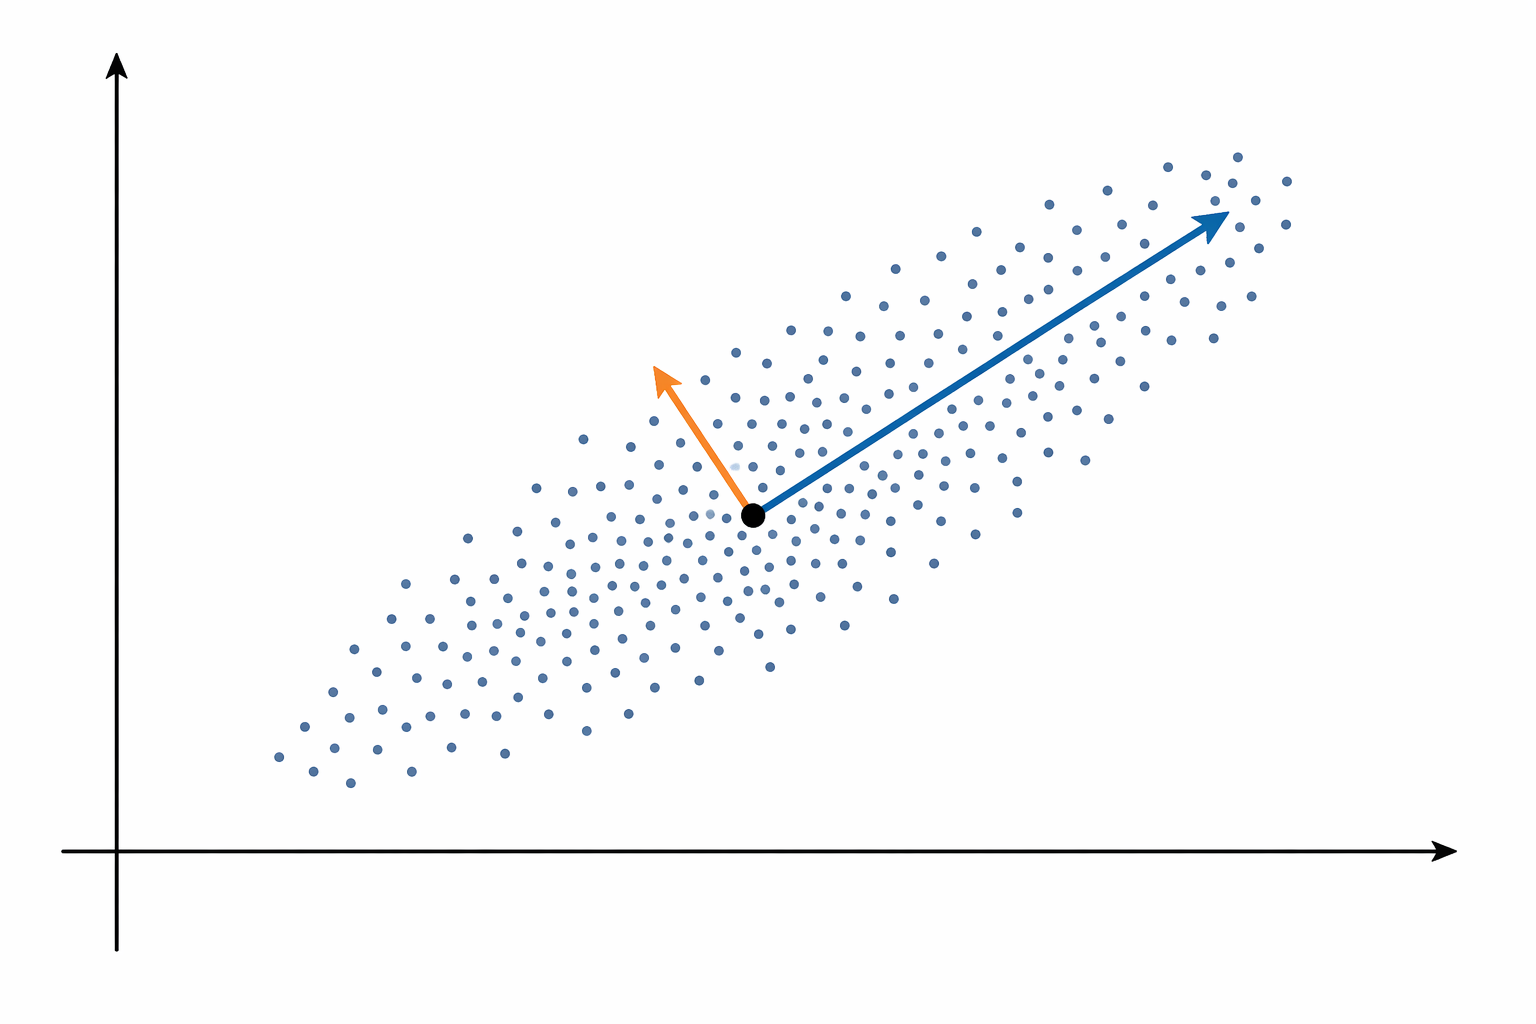
\includegraphics[width=0.86\textwidth]{figures/pca/principal-directions.png}
  \caption{A data cloud has different variances in different directions. PCA chooses the first direction along the largest spread of the centered cloud, then chooses orthogonal directions that explain the remaining variance.}
\end{figure}

The iris example in the slides is a useful starting intuition. A flower is measured by several numerical attributes, and scatter plots of pairs of attributes already show some structure. PCA generalizes this search beyond pairwise plots: it finds linear combinations of the original attributes that can reveal separation, compression, or nuisance variation.

\subsection{Moments of the Data Cloud}

PCA is built from the first two empirical moments of the observations. The sample mean is the center of mass,
\[
  m = \frac{1}{p}\sum_{\alpha=1}^{p} x^{(\alpha)}.
\]
The covariance matrix records the centered second moments:
\[
  C_{ij}
  =
  \frac{1}{p}\sum_{\alpha=1}^{p}
  \bigl(x_i^{(\alpha)} - m_i\bigr)
  \bigl(x_j^{(\alpha)} - m_j\bigr).
\]
For centered data, where $m=0$, this simplifies to
\[
  C_{ij}
  =
  \frac{1}{p}\sum_{\alpha=1}^{p}
  x_i^{(\alpha)}x_j^{(\alpha)}.
\]

The diagonal entries $C_{ii}$ are variances of individual variables. The off-diagonal entries $C_{ij}$ are covariances between variables. The matrix is symmetric, so $C_{ij}=C_{ji}$. A zero covariance means two variables are uncorrelated, but it does not prove statistical independence; nonlinear dependence can remain invisible to a second-order method.

\subsection{Variance Along a Complex Feature}

Let $e_a$ be a unit vector in feature space. The induced feature value is
\[
  u_a^{(\alpha)} = e_a^{\mathsf{T}}x^{(\alpha)}.
\]
Its mean is
\[
  m_a
  =
  \frac{1}{p}\sum_{\alpha=1}^{p}u_a^{(\alpha)}
  =
  e_a^{\mathsf{T}}m.
\]
Its variance is
\[
  \sigma_a^2
  =
  \frac{1}{p}\sum_{\alpha=1}^{p}
  \bigl(u_a^{(\alpha)} - m_a\bigr)^2
  =
  e_a^{\mathsf{T}} C e_a.
\]
This identity is the hinge of the lecture: the covariance matrix determines the variance of the data along every possible direction. Once $C$ is known, PCA can compare all candidate directions without returning to the raw data points.

\subsection{The Principle of Maximal Variance}

The first principal component is the unit direction with maximal projected variance:
\[
  e_1
  =
  \operatorname*{arg\,max}_{\|e\|=1} e^{\mathsf{T}}Ce.
\]
The unit-length constraint is essential. Without it, the variance could be made arbitrarily large by scaling $e$. Introducing a Lagrange multiplier gives
\[
  \mathcal{L}(e,\lambda)
  =
  e^{\mathsf{T}}Ce
  -
  \lambda\bigl(e^{\mathsf{T}}e - 1\bigr).
\]
Setting the derivative with respect to $e$ to zero yields
\[
  Ce = \lambda e.
\]
Thus the principal components are the normalized eigenvectors of the covariance matrix. The variance along a principal component is the corresponding eigenvalue:
\[
  \sigma_a^2 = e_a^{\mathsf{T}}Ce_a = \lambda_a.
\]

\paragraph{PCA eigenproblem.}
\[
  Ce_a = \lambda_a e_a,
  \qquad
  \lambda_1 \ge \lambda_2 \ge \dots \ge \lambda_N.
\]

The eigenvectors give the principal directions. The eigenvalues rank those directions by explained variance.

\subsection{Properties of Principal Components}

Because the covariance matrix is real and symmetric, its eigenvectors form an orthonormal basis:
\[
  e_i^{\mathsf{T}}e_j = \delta_{ij}.
\]
Ordering the eigenvalues from largest to smallest orders the corresponding eigenvectors from most variable to least variable. The first principal component points along the largest variance in the full space. The second points along the largest remaining variance in the subspace orthogonal to the first, and so on.

\subsubsection{Optimal Linear Dimensionality Reduction}

Any observation can be represented in the principal-component basis:
\[
  x = a_1e_1 + a_2e_2 + \dots + a_Ne_N,
  \qquad
  a_j = e_j^{\mathsf{T}}x.
\]
Keeping only the first $M$ terms gives the rank-$M$ PCA approximation
\[
  \tilde{x}
  =
  a_1e_1 + a_2e_2 + \dots + a_Me_M.
\]
Among all $M$-dimensional linear projections, this choice minimizes the mean-squared reconstruction error:
\[
  E
  =
  \frac{1}{p}\sum_{\alpha=1}^{p}
  \bigl\|x^{(\alpha)}-\tilde{x}^{(\alpha)}\bigr\|^2
  =
  \sum_{j=M+1}^{N} \lambda_j.
\]
In words, the error is the variance left behind in the discarded principal components.

\begin{figure}[htbp]
  \centering
  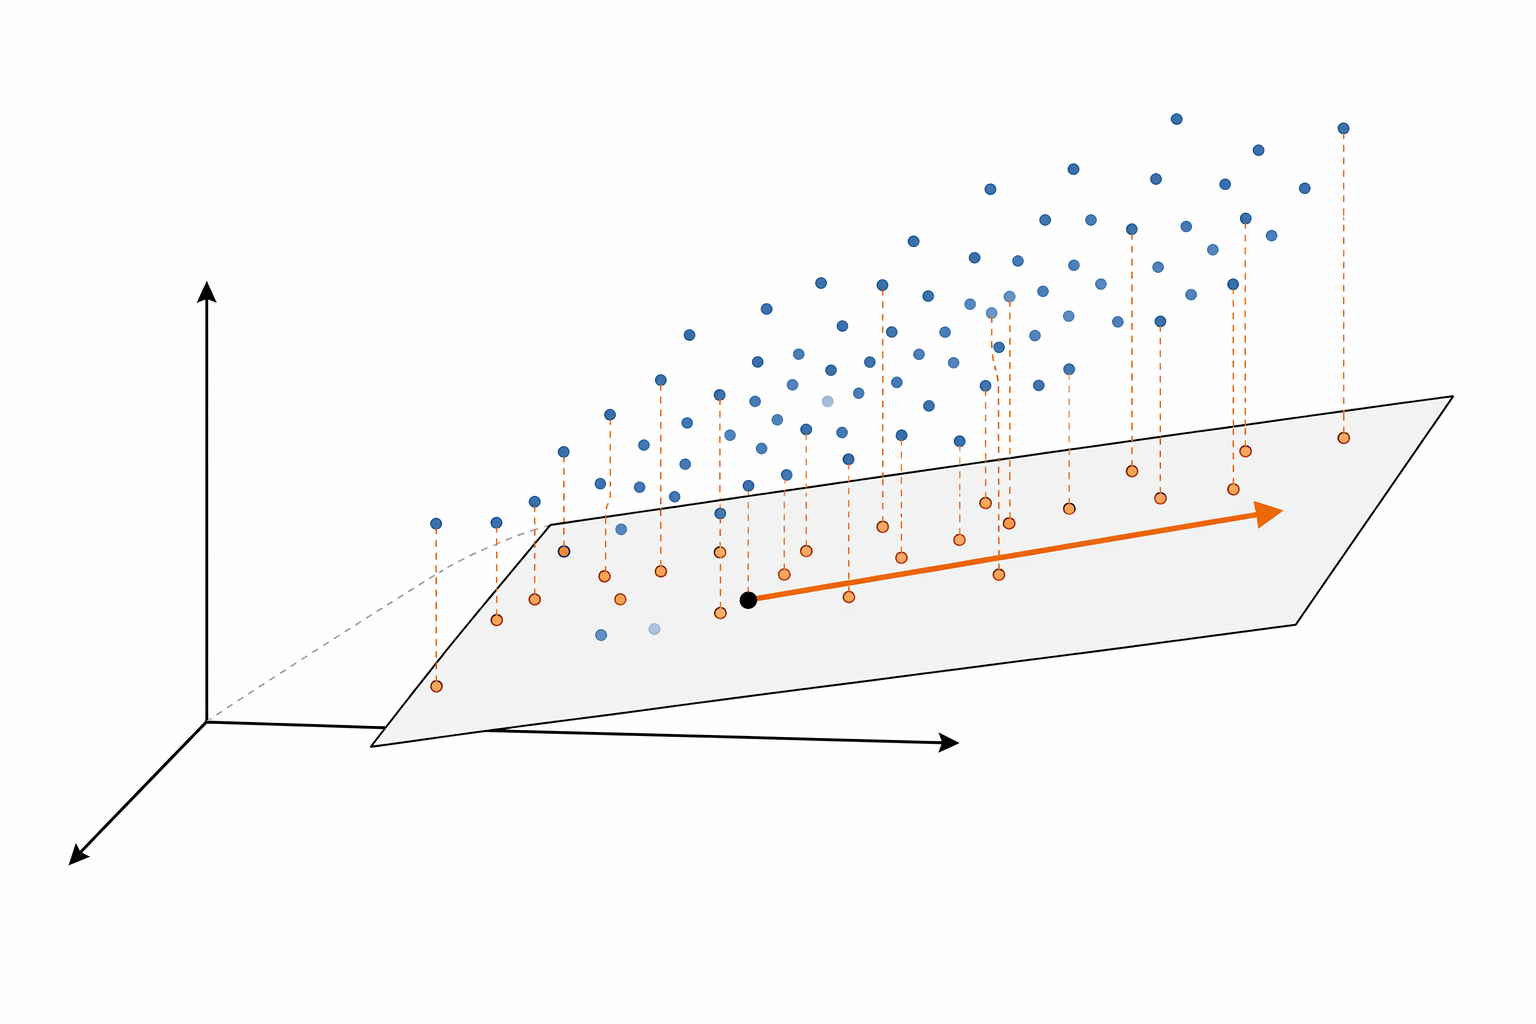
\includegraphics[width=0.88\textwidth]{figures/pca/projection-subspace.png}
  \caption{Dimensionality reduction by projection. PCA keeps the principal subspace that preserves the largest variance and leaves only the orthogonal residual as reconstruction error.}
\end{figure}

\subsubsection{Decorrelation}

Let
\[
  M = \bigl(e_1,e_2,\dots,e_N\bigr)
\]
be the matrix whose columns are the principal components. In this basis, the covariance matrix is diagonal:
\[
  M^{\mathsf{T}}CM
  =
  \Lambda
  =
  \operatorname{diag}(\lambda_1,\lambda_2,\dots,\lambda_N).
\]
The transformed features are therefore uncorrelated. This is why PCA is often used before regression, classification, clustering, or visualization: it rotates the coordinate system into axes that separate second-order variation cleanly.

\subsubsection{Whitening}

Variance is scale sensitive. If one input dimension is measured in much larger units than another, a variance criterion may prioritize scale rather than structure. PCA therefore only makes direct sense when feature scales are comparable, or after suitable normalization.

After decorrelation, whitening rescales every principal direction to unit variance:
\[
  v^{(\alpha)}
  =
  \Lambda^{-1/2}M^{\mathsf{T}}x^{(\alpha)}.
\]
The result has covariance equal to the identity matrix. Whitening removes both linear correlations and unequal variances, making the transformed representation scale-standardized.

\begin{figure}[htbp]
  \centering
  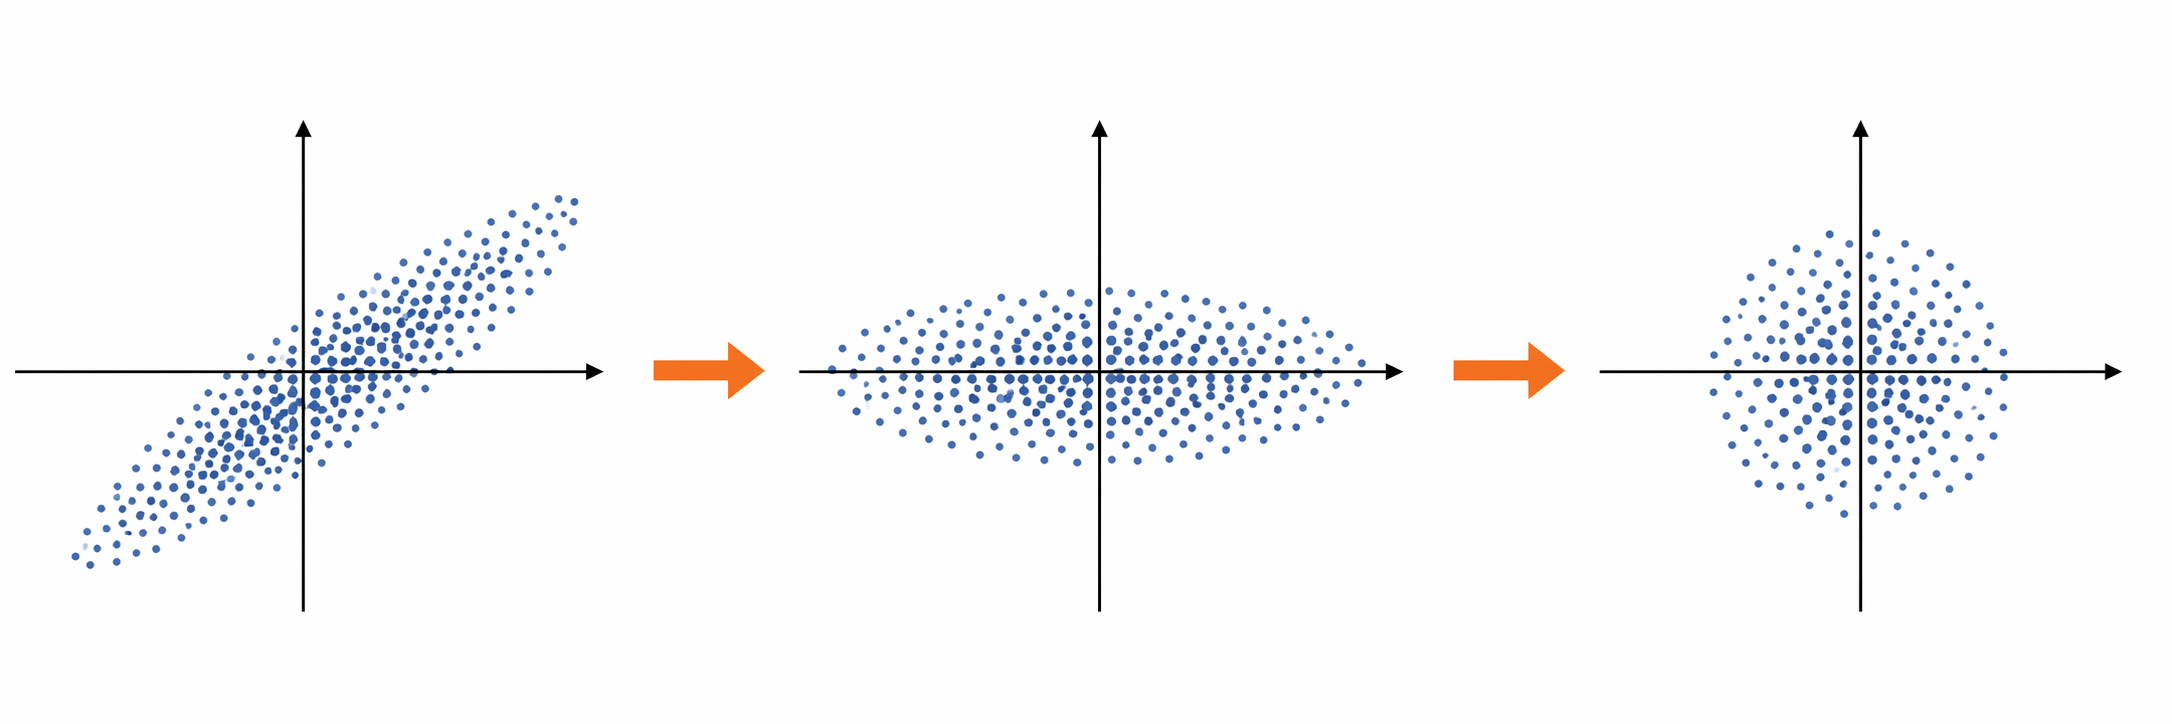
\includegraphics[width=0.92\textwidth]{figures/pca/decorrelation-whitening.png}
  \caption{PCA first rotates an elongated data cloud into its eigenbasis, where the covariance is diagonal. Whitening then rescales the axes so the transformed cloud has unit variance in every retained direction.}
\end{figure}

\subsection{Applications and Interpretations}

\subsubsection{Iris Data}

The iris slides use a familiar biological dataset to motivate projection methods. Pairwise scatter plots can show partial separation between setosa, versicolor, and virginica, but PCA asks for the strongest directions in the full feature space rather than inspecting every pair of raw features. This makes it a compact exploratory tool when there are more variables than can be inspected directly.

\subsubsection{Leptograpsus Crab Measurements}

The Leptograpsus example is more explicitly about complex features. Each crab is described by five measurements: frontal lobe size, rear width, carapace length, carapace width, and body depth. PCA forms linear combinations of these elementary features. The leading component can capture overall size, while later components may align with sex- or species-related variation if those factors explain substantial covariance structure.

This example also warns against overinterpreting components. A principal component is a direction chosen by variance, not by semantics. A component may become interpretable as ``size'' or ``sex'' only after examining its loadings and how observations project onto it.

\subsubsection{Outlier Detection}

The lecture also points out a less obvious use of PCA: components with the smallest eigenvalues can help detect outliers or novel features. A normal data point should not vary much along a low-variance direction. A large projection onto such a direction can therefore indicate an unusual observation, a measurement artifact, or a rare structure not captured by the dominant modes.

\subsection{Computational Notes and Extensions}

PCA is linear, second-order, and variance-based. This is both its strength and its limitation. It is efficient, interpretable, and useful for preprocessing, dimensionality reduction, and compression. But very large covariance matrices can be numerically unstable or expensive, and second-order structure cannot capture every kind of dependence.

The slide summary points to two algorithmic routes for extracting leading principal components: Hebbian learning and the power method. Both are useful when the largest eigenvectors matter more than the full eigenspectrum. It also points forward to extensions. Kernel PCA replaces the raw feature space with nonlinear features, while probabilistic PCA and factor analysis add an explicit generative model. Later methods such as ICA change the objective from decorrelation to statistical independence.

\paragraph{Summary.}
PCA begins with the covariance matrix and asks which unit directions maximize projected variance. The solution is the eigenbasis of $C$: eigenvectors are principal components, and eigenvalues measure explained variance. Keeping the leading components gives the optimal linear low-dimensional reconstruction, rotating into the eigenbasis decorrelates the features, and whitening additionally rescales them to unit variance. The method is simple and powerful, but it remains linear and variance-based, so later MI2 methods relax or extend these assumptions.
